\documentclass[letter]{article}

%% Language and font encodings
\usepackage[english]{babel}
\usepackage[utf8x]{inputenc}
\usepackage[T1]{fontenc}
\usepackage{enumitem}
\usepackage{fancyhdr}
\pagestyle{fancy}

%% Useful packages
\usepackage{amsmath, amsthm, amssymb}
\usepackage{graphicx}
\newtheoremstyle{case}{}{}{}{}{}{:}{ }{}
\theoremstyle{case}
\newtheorem{case}{}


\title{HW Template}
\author{Nicholas Silva Tee}
\lhead{Homework Template}



\begin{document}

\subsection*{Problem 1.1}
\textbf{a.} $M_1: q_1$ $M_2: q_1$ \\
\textbf{b.} $M_1: \{q_2\}$ $M_2: \{q_1,q_4\}$\\
\textbf{c.} $M_1: q_1 \rightarrow q_2 \rightarrow q_3 \rightarrow q_1 \rightarrow q_1$ 
$M_2: q_1 \rightarrow q_1 \rightarrow q_1 \rightarrow q_2 \rightarrow q_4$\\
\textbf{d.} $M_1:$ no $M_2:$ yes\\
\textbf{e.} $M_1:$ no $M_2:$ yes\\

\subsection*{Problem 1.2}
$M_1$ definition: \\
$Q: \{q_1,q_2,q_3\}$ \\
$\Sigma: \{a,b\}$ \\
$\delta$ can be shown as: \\
\begin{table}[h!]
\begin{tabular}{l|ll}
 &$a$  &$b$  \\ \hline
$q_1$ &$q_2$  &$q_1$  \\
$q_2$ &$q_3$  &$q_3$  \\
$q_3$ &$q_2$  &$q_1$ 
\end{tabular}
\end{table} \\
$q_1$ is the start state \\
$F: \{q_2\}$

\subsection*{Problem 1.3}
\begin{figure}[h!]
	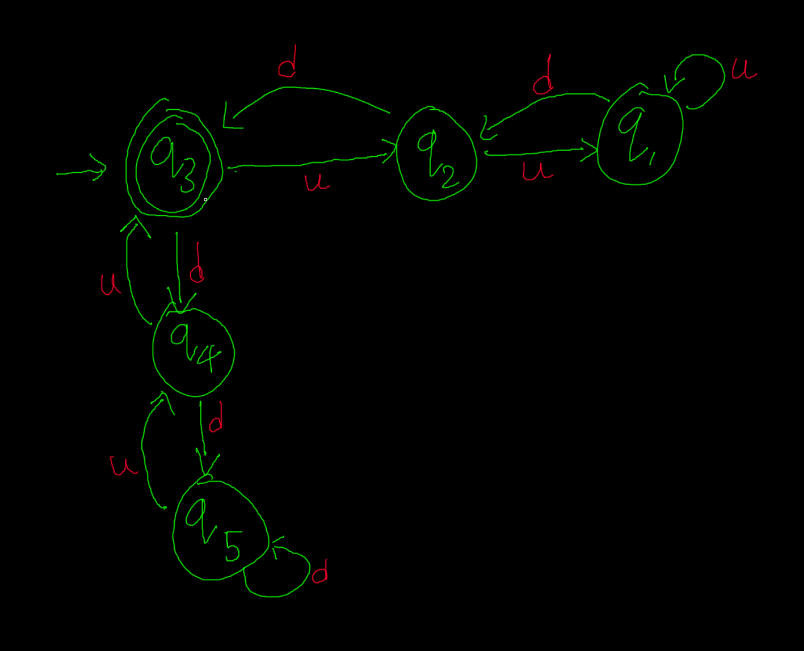
\includegraphics[scale=0.4]{model1.png}
\end{figure}

\newpage

\subsection*{Problem 1.4}
\textbf{a.}
\begin{figure}[h!]
	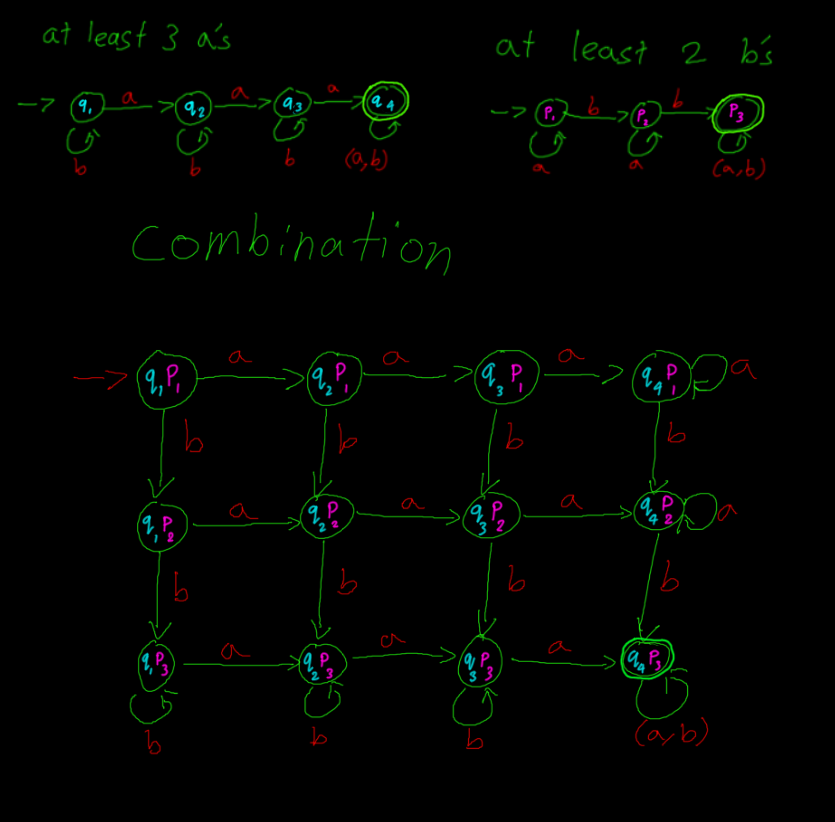
\includegraphics[scale=0.4]{4a.png}
\end{figure} 

\textbf{c.} 
\begin{figure}[h!]
	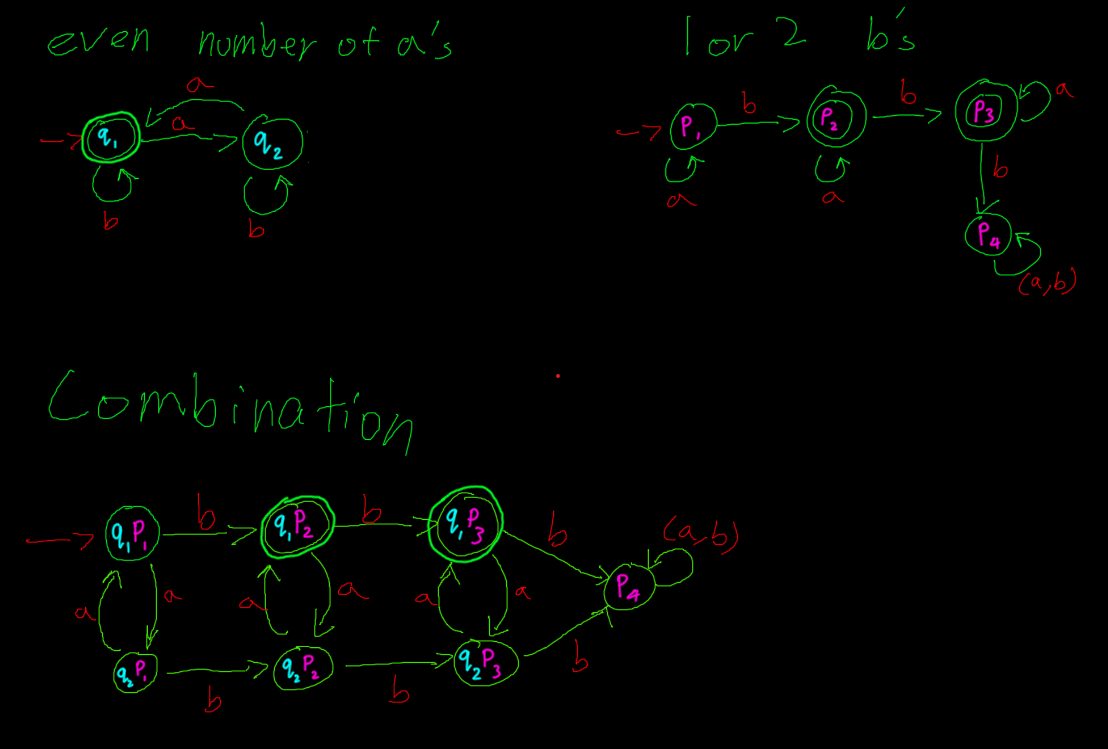
\includegraphics[scale=0.4]{4c.png}
\end{figure} 

\textbf{f.}
\begin{figure}[h!]
	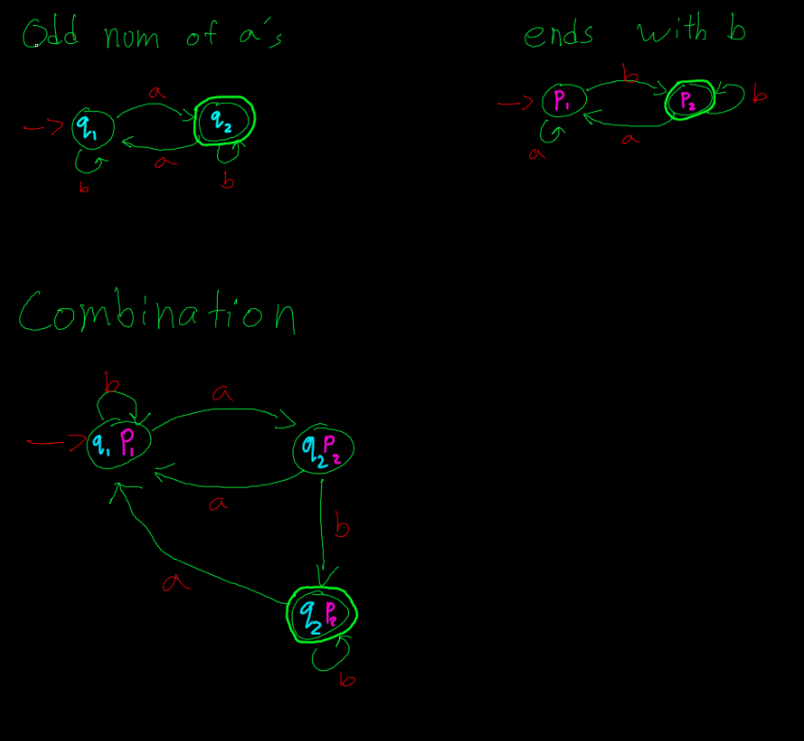
\includegraphics[scale=0.4]{4f.png}
\end{figure} 

\textbf{g.}
\begin{figure}[h!]
	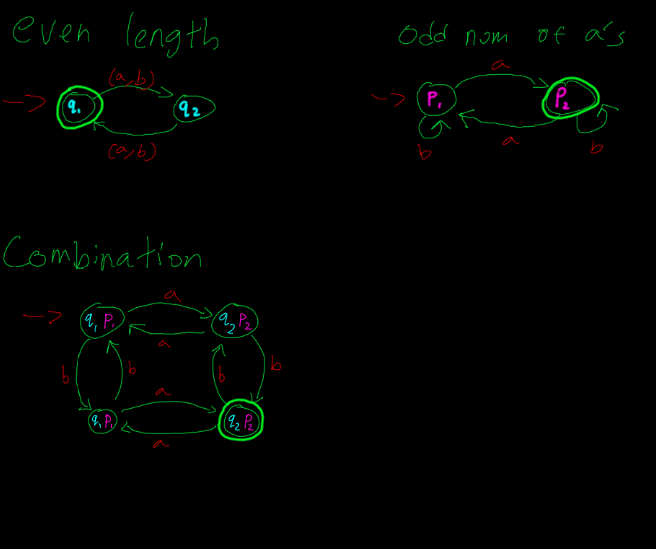
\includegraphics[scale=0.4]{4g.png}
\end{figure}

\newpage

\subsection*{Problem 1.5}
\textbf{c.}
\begin{figure}[h!]
	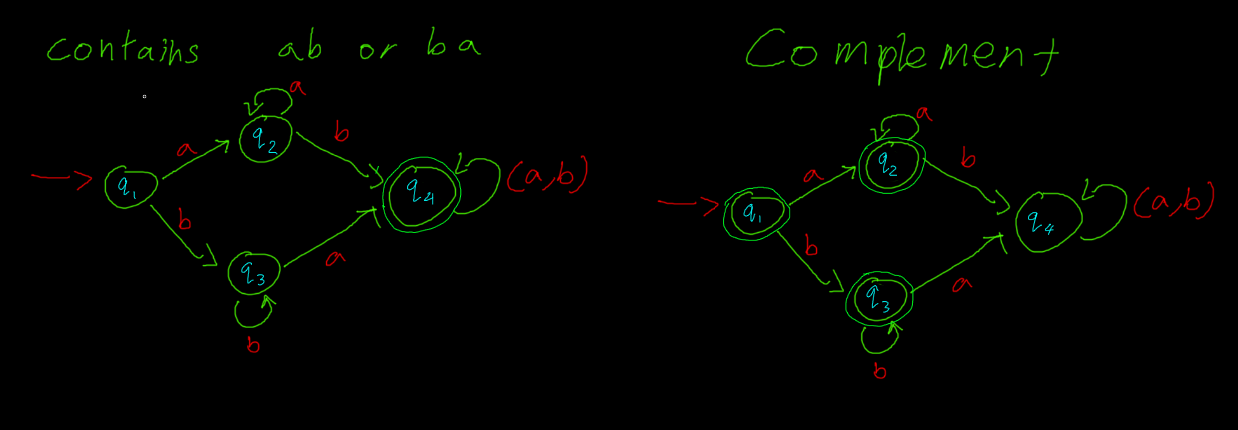
\includegraphics[scale=0.4]{5c.png}
\end{figure}

\textbf{d.}
\begin{figure}[h!]
	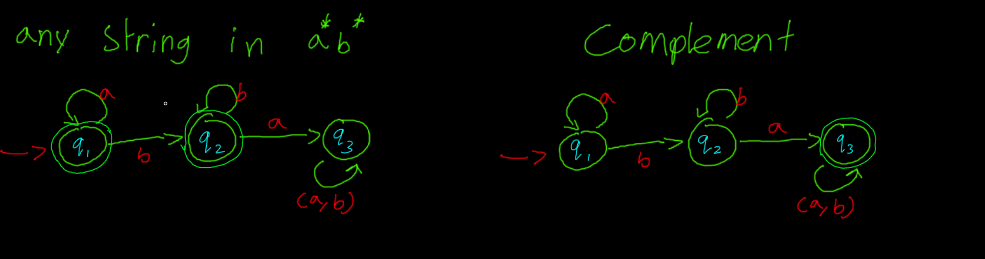
\includegraphics[scale=0.4]{5d.png}
\end{figure}

\textbf{e.}
\begin{figure}[h!]
	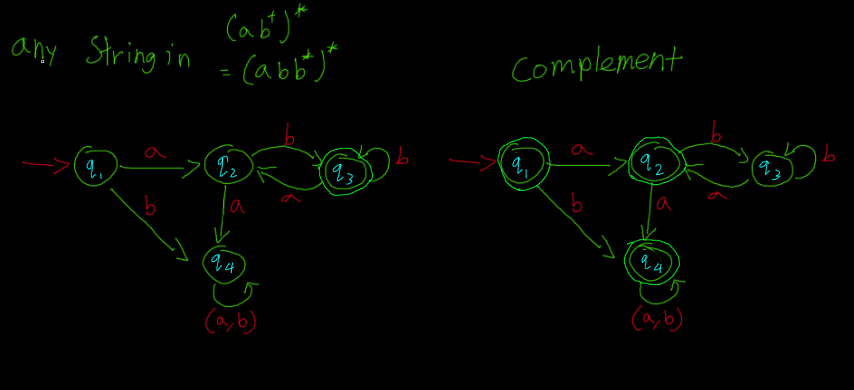
\includegraphics[scale=0.4]{5e.png}
\end{figure}

\newpage

\textbf{f.}
\begin{figure}[h!]
	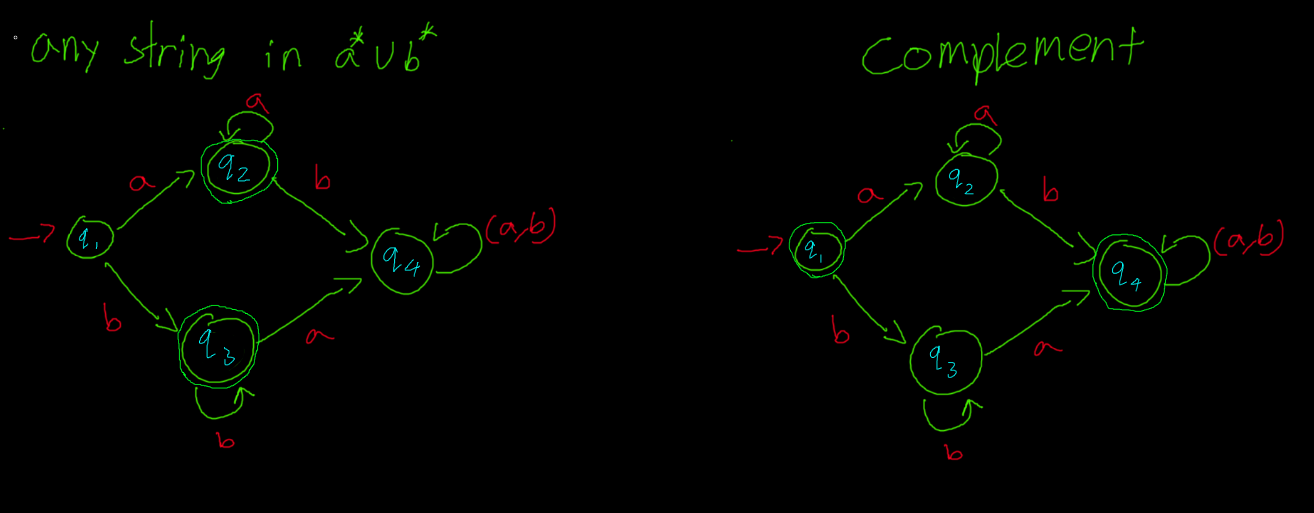
\includegraphics[scale=0.4]{5f.png}
\end{figure}

\textbf{g.}
\begin{figure}[h!]
	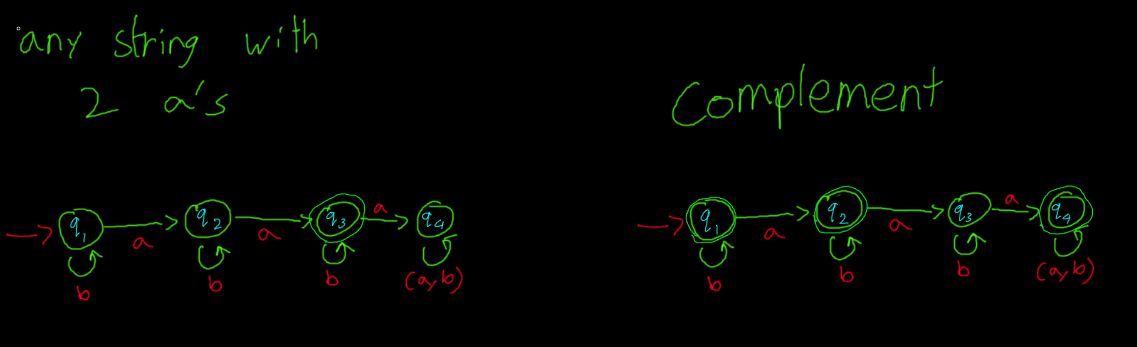
\includegraphics[scale=0.4]{5g.png}
\end{figure}

\textbf{h.}
\begin{figure}[h!]
	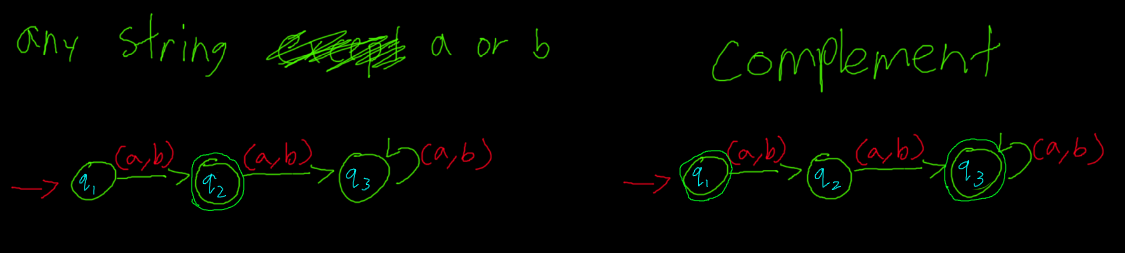
\includegraphics[scale=0.4]{5h.png}
\end{figure}

\newpage
\subsection*{Problem 1.6}
\textbf{a.}
\begin{figure}[h!]
	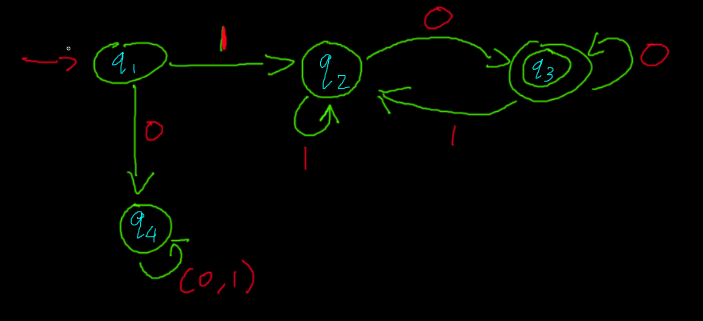
\includegraphics[scale=0.4]{6a.png}
\end{figure}

\textbf{b.}
\begin{figure}[h!]
	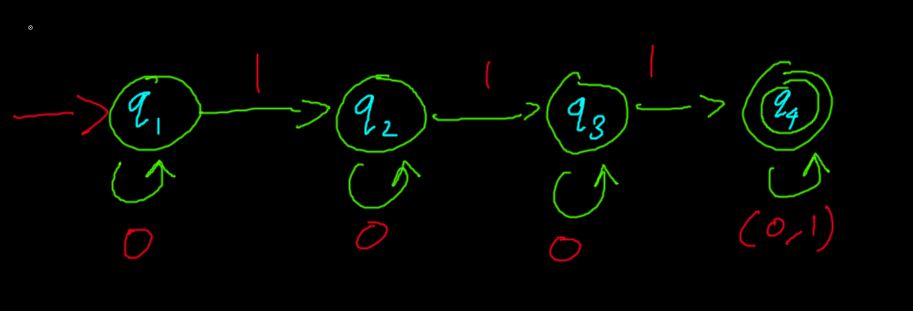
\includegraphics[scale=0.4]{6b.png}
\end{figure}

\textbf{c.}
\begin{figure}[h!]
	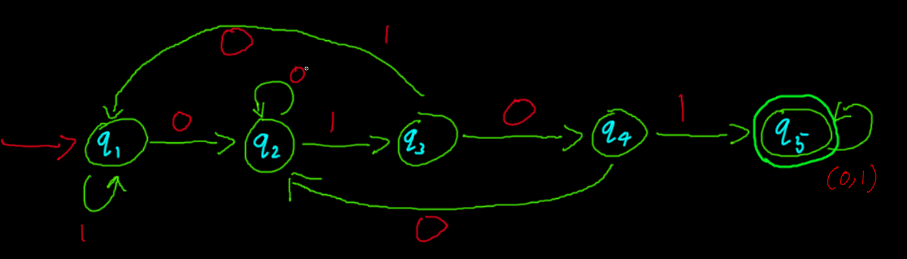
\includegraphics[scale=0.4]{6c.png}
\end{figure}
\newpage
\textbf{d.}
\begin{figure}[h!]
	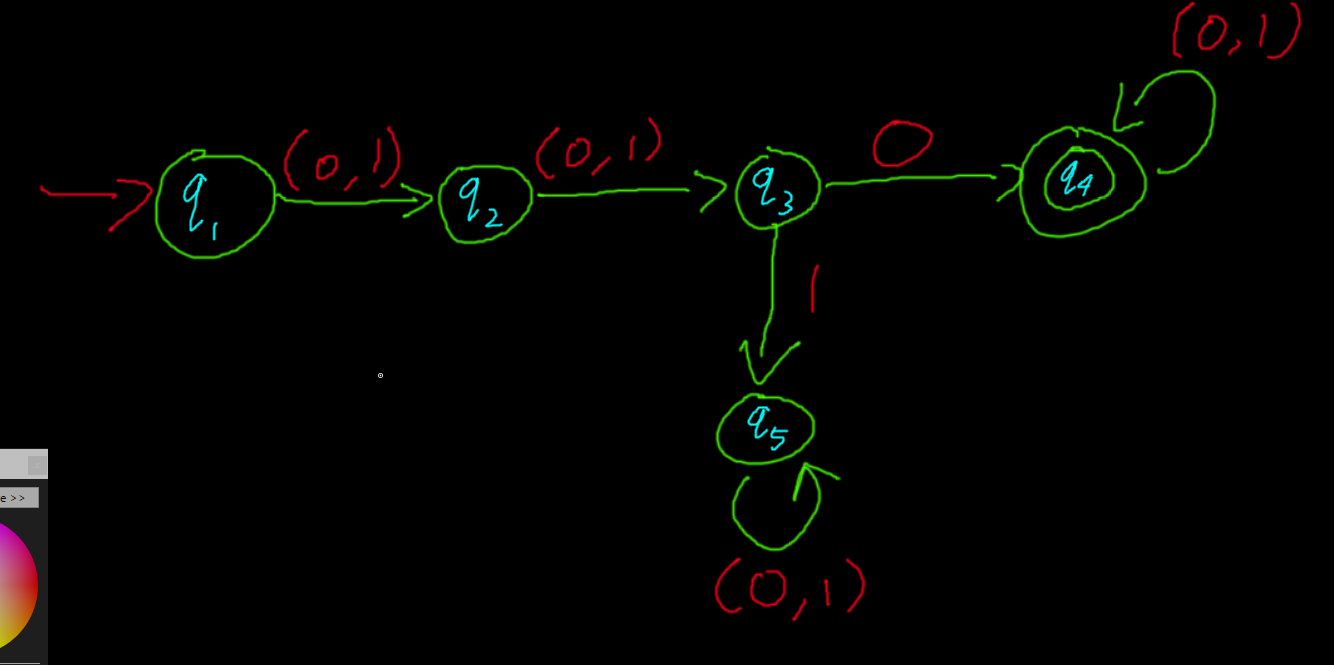
\includegraphics[scale=0.4]{6d.png}
\end{figure}

\textbf{e.}
\begin{figure}[h!]
	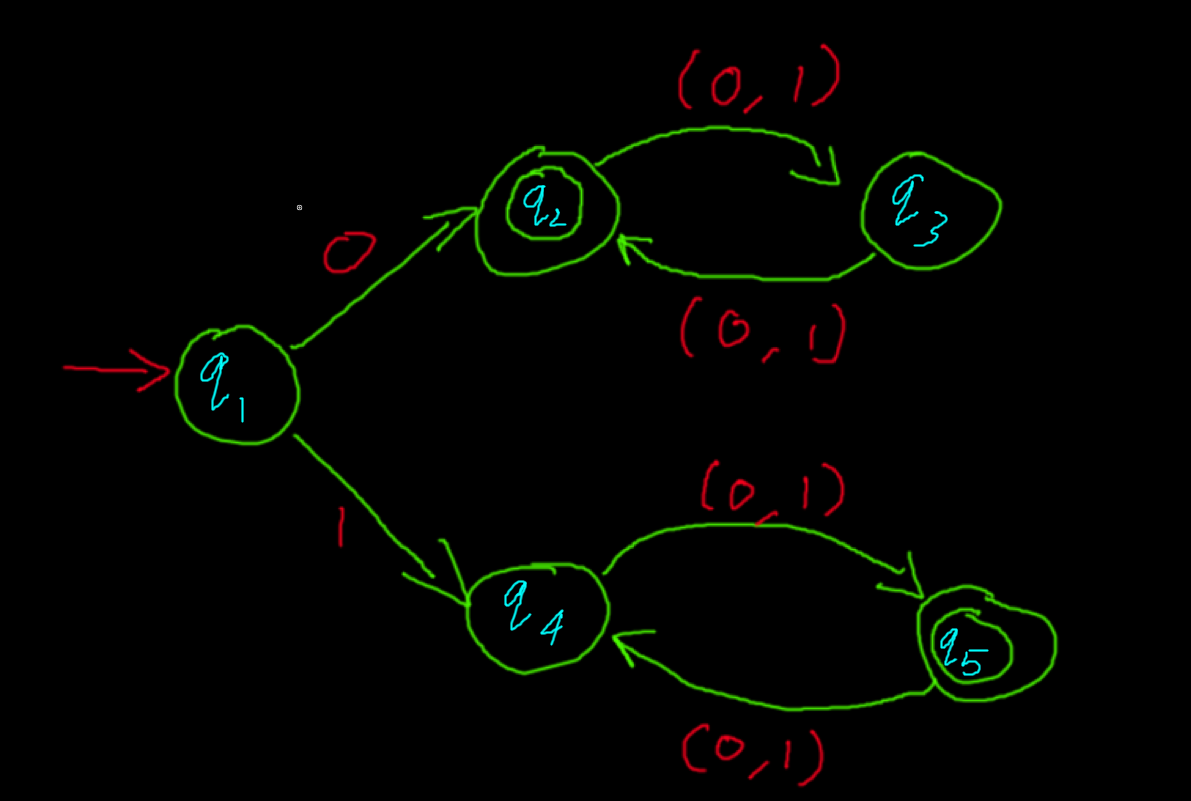
\includegraphics[scale=0.4]{6e.png}
\end{figure}
 \newpage
\textbf{f.}
\begin{figure}[h!]
	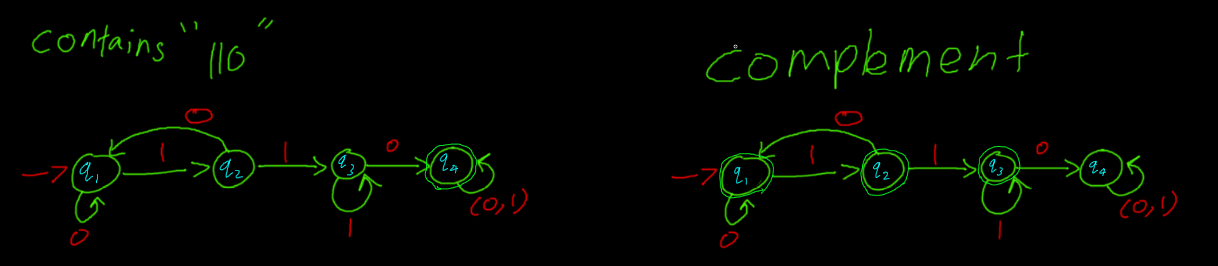
\includegraphics[scale=0.4]{6f.png}
\end{figure}

\textbf{g.}
\begin{figure}[h!]
	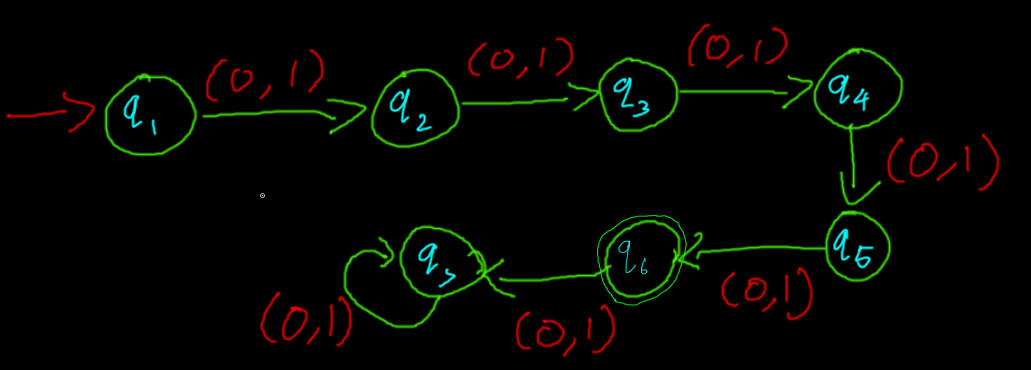
\includegraphics[scale=0.4]{6g.png}
\end{figure}

\textbf{h.}
\begin{figure}[h!]
	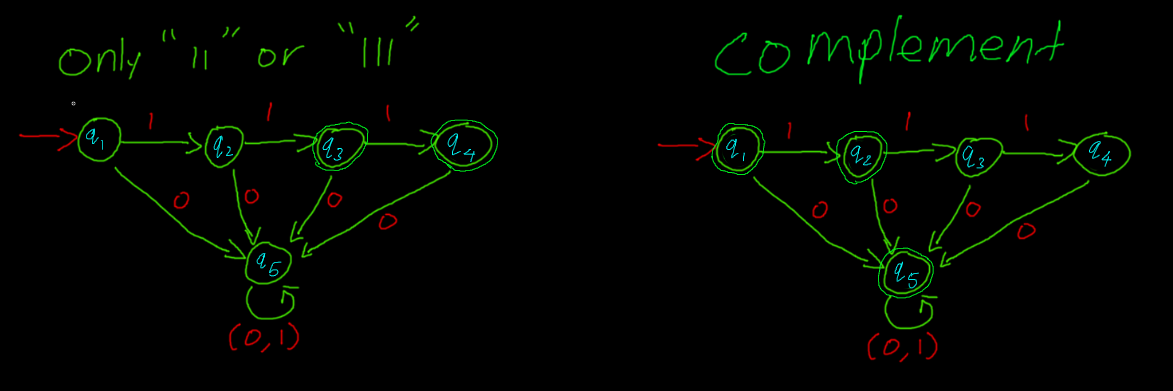
\includegraphics[scale=0.4]{6h.png}
\end{figure}
\newpage
\textbf{i.}
\begin{figure}[h!]
	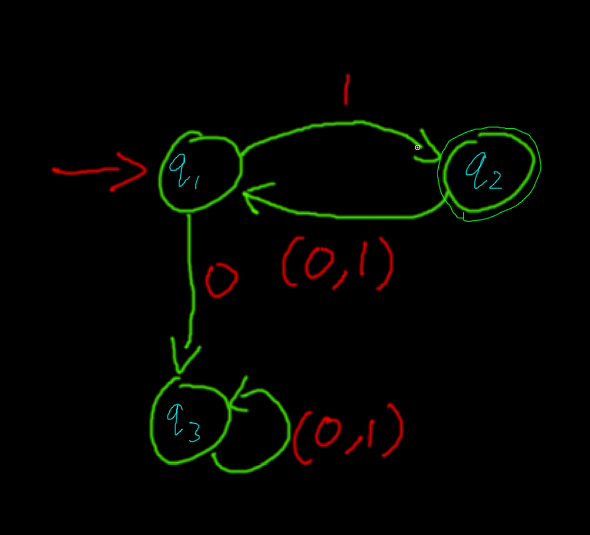
\includegraphics[scale=0.4]{6i.png}
\end{figure}

\textbf{j.}
\begin{figure}[h!]
	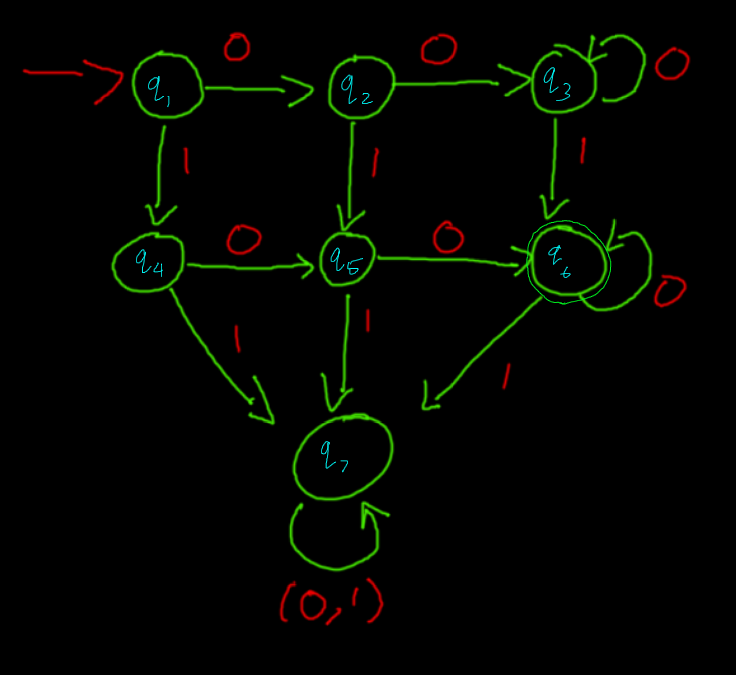
\includegraphics[scale=0.4]{6j.png}
\end{figure}
\newpage
\textbf{k.}
\begin{figure}[h!]
	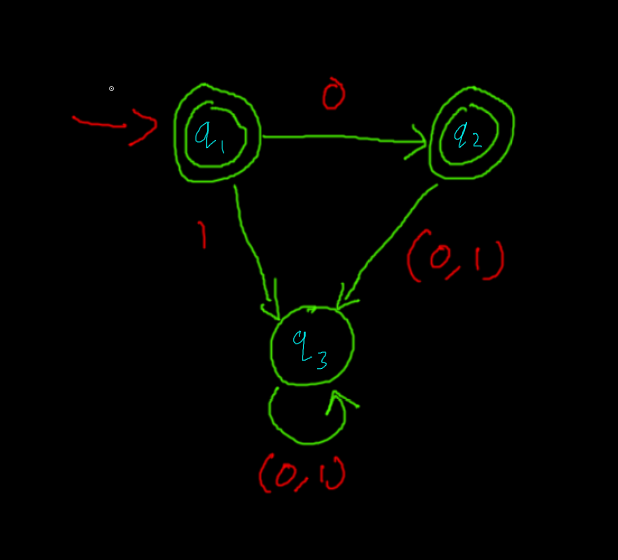
\includegraphics[scale=0.4]{6k.png}
\end{figure}

\textbf{l.}
\begin{figure}[h!]
	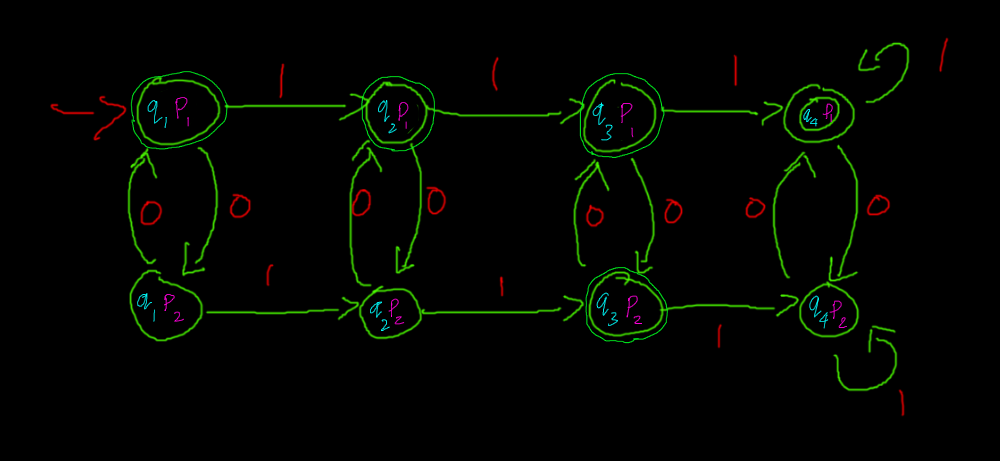
\includegraphics[scale=0.4]{6l.png}
\end{figure}

\textbf{m.}
\begin{figure}[h!]
	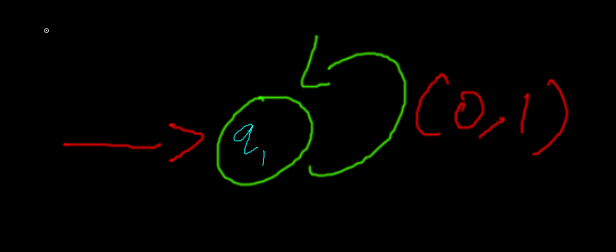
\includegraphics[scale=0.4]{6m.png}
\end{figure}
\newpage
\textbf{n.}
\begin{figure}[h!]
	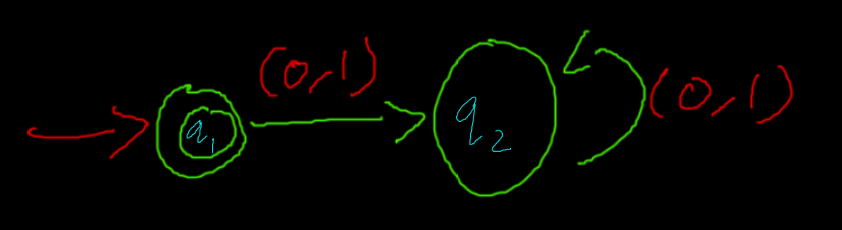
\includegraphics[scale=0.4]{6n.png}
\end{figure}

\end{document}










